Im folgenden werden die verschiedenen Benutzeroberflächen gezeigt und die grundlegende Architektur festgelegt.

\subsection{Benutzerschnittstellen}



\subsection{Architektur}
Das Klassendiagramm (siehe Abbildung \ref{uml}) zeigt den Aufbau der Anwendung. Die einzelnen Klassen und deren Funktionen sind im folgenden erklärt.

\subsubsection*{ImageManager}
Die Klasse ImageManager hat die Aufgabe aus einer Datenquelle alle SpotImages zu erzeugen und diese zu verwalten.

\subsubsection*{SpotImage}
Ein SpotImage definiert ein spezielles Fehlerbild mitsamt seinen geographischen Koordinaten, Titel, Beschreibungstext und den eigentlichen Fehlern (Klasse Difference). Sie bietet über die Funktion ''doesHitWith'' die Möglichkeit anhand der Angabe einer xy-Koordinate festzustellen ob dort ein Fehler im Bild existiert. Diese Funktion wird benötigt wenn der Benutzer auf das Bild, um zu überprüfen ob dort auch wirklich ein Fehler versteckt ist.

\subsubsection*{Difference}
Die Klasse Difference stellt einen einzelnen Fehler in einem SpotImage dar. Dieser wird durch seine Position im Bild (xy-Koordinate) und dessen Größe (Breite und Höhe) definiert.

\subsubsection*{MapViewController}
Der MapViewController ist für den View zuständig, der die Weltkarte und die SpotImages anzeigt.

\subsubsection*{ImageViewController}
Das Anzeigen des im MapViewController ausgewählten SpotImage geschieht im View des ImageViewController. Der ImageViewController besitzt daher eine Referenz auf das gerade aktive SpotImage. Alle aufgedeckten Fehler werden temporär gemerkt um dem Spieler zu zeigen wie viele Fehler noch zu finden sind.

\subsubsection*{AboutViewController}
Für die Anzeige einer Kurzanleitung für das Spiel ist der AboutViewController zuständig.


\begin{figure}[H]
  \centering
  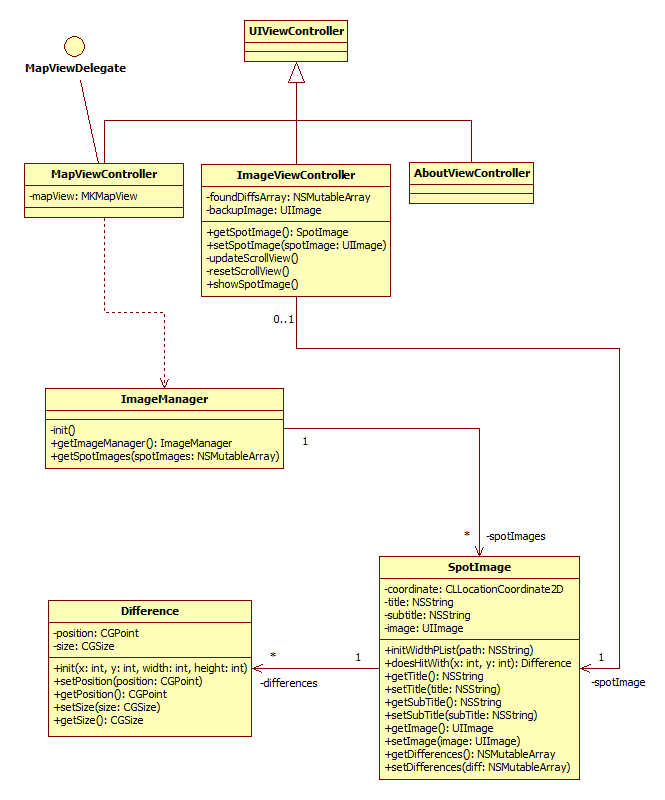
\includegraphics[width=1.0\textwidth]{bilder/uml.png}
  \caption{UML-Klassendiagramm}
  \label{uml}
\end{figure}